\chapter{Background}

This project is quite broad and combines knowledge coming from different fields.
Here we cover the theoretical background required to understand it.

\section{Cyber-Physical Systems}

The field of CPS, Cyber-Physical Systems, is relatively new: the name was coined and started gaining ground only in the first decade of the 2000s.
The knowledge employed in this field, however, comes from well-known disciplines: CPS is, in fact, a highly interdisciplinary area where Physics, Control Theory, Embedded Systems, Formal Verification and Robotics.

Despite the recent foundation of this field, the first medical devices that can be classified as CPS are quite dated: pace-makers and insulin-pumps, for instance, were invented around the '60s.
Due to the increasing computational power of the controllers classified as Edge Computing \cite{edge_comp_2016} and to the new possibilities given by the advent of the Internet of Things, we are going to hear about CPS new fields of application: they are already effectively used in growing fields like automotive, manufacturing, energy management and in any other field that involves the employment of robots \cite{Sanislav_Miclea_2012}.

Each of this fields deals with \textit{Complex Systems} in which \textbf{continuous}, \textbf{discrete} and \textbf{stochastic} processes are involved.

\subsection{Definition}
As the name suggests, a Cyber-Physical System is composed of two parts:
\begin{itemize}
  \item the "\textbf{cyber}" one is a computational system that processes logical operations,
  \item the "\textbf{physical}" one is the real phenomenon that we are modelling.
\end{itemize}
We define it CPS only when the two components are deeply interconnected by some communication devices that can affect each other's state.

The major difference between the two components is their way of dealing with time.
The \textit{cyber} part operates in a discrete time-scale where the internal state of the model is governed by the execution of algorithms.
The \textit{physical} part, instead, lives in a continuous time-scale where the model's state evolves according to the physical laws of nature.

The communication between the two components of the CPS takes place through \textbf{transducers}, allowing the exchange of information between them.
This allows the two parts to co-evolve simultaneously following their respective rules: the instructions of the algorithm for the \textit{cyber} part and physical laws the \textit{physical} one.

\textbf{Sensors} are transducers that discretize an analog signal, therefore, they allow the flow of information from the \textit{physical} part to the \textit{cyber} part.
For instance, we call \textit{sensor} whatever is able to digitally measure a property of the physical world: thermometers, photoresistors, camera sensors, etc.

\textbf{Actuators}, instead, are transducers that use a digital input to transform the physical world.
They work in the exact opposite way with respect to \textit{sensors}, in fact, they allow the information from the \textit{cyber} part to flow toward the \textit{physical} one.
Examples of actuators are all those devices that, given a digital input, can produce an observable change in the world: motors, speakers, electromagnets, etc.

\begin{figure}[H]
	\centering
	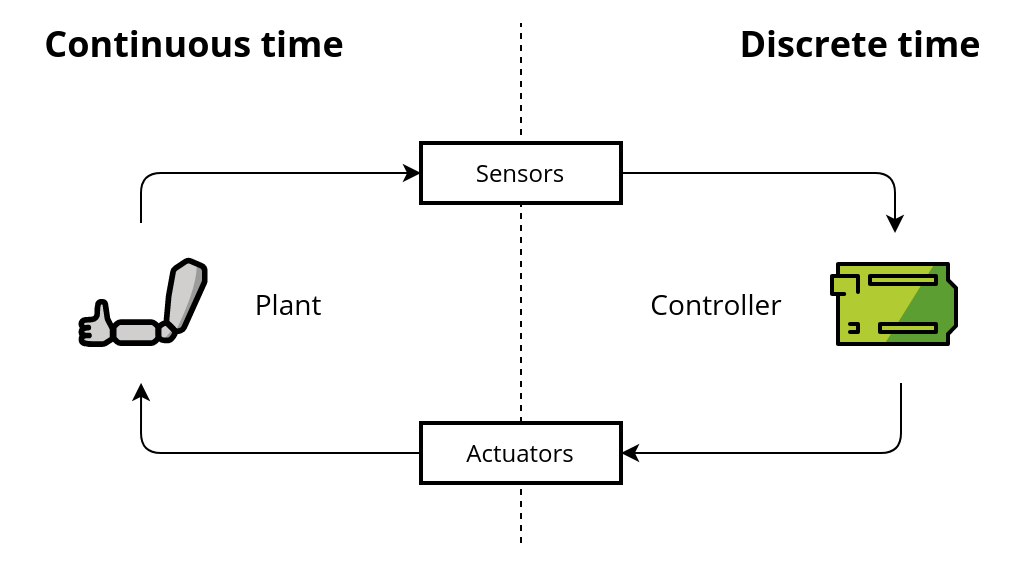
\includegraphics[width=11cm, keepaspectratio]{img/2_1_cps.png}
	\caption{The two components of a CPS interact through sensors and actuators, these allow them to exchange information and act as a single system.}
\end{figure}

The communication between the two parts is fundamental because a CPS acts as a whole due to the constant flow of information that allows the two parts to adapt to each other.
We are now going to describe a practical example of CPS: the \textit{cruise-control}, whose aim is to keep constant the speed of a vehicle.

\subsection{Physical component}
In the cruise-control example, the vehicle and its dynamic represent the physical part of the CPS.
This part is often referred to as the \textbf{plant}.
We call \textit{state} a specific configuration of the variables describing the model's properties we are interested in.
For instance, in the cruise-control problem, the \textit{state} is composed of the vehicle's speed $v$ and the \textit{steepness} of the road $\theta$.
The \textit{plant} evolves its \textit{state} in time according to the physical laws involved.

\begin{figure}[H]
	\centering
	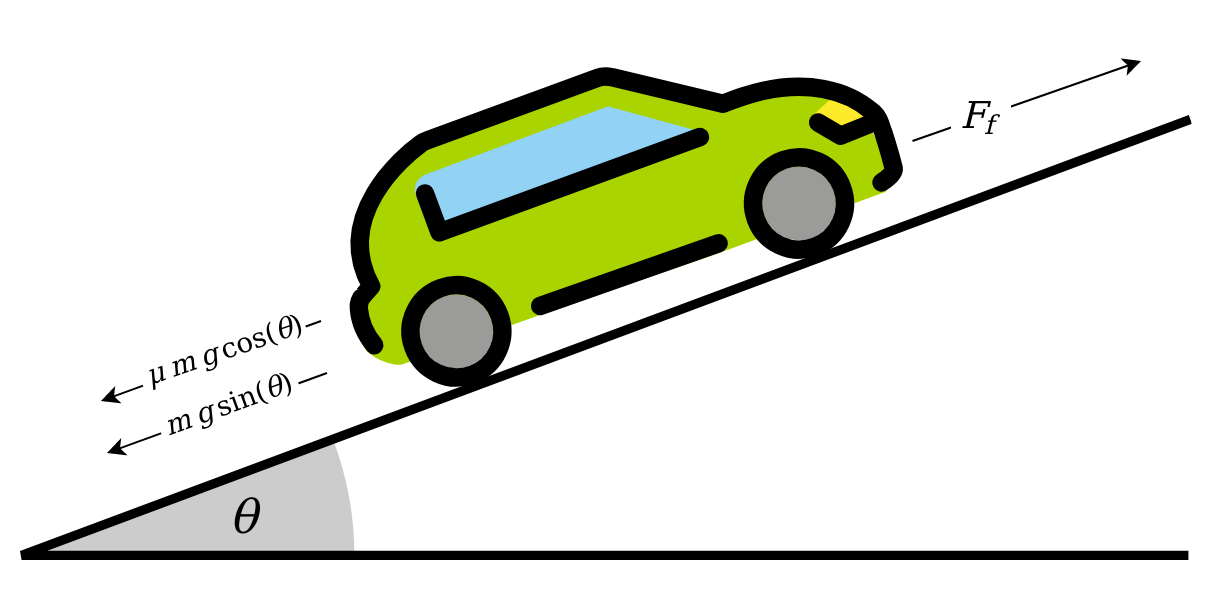
\includegraphics[width=11cm, keepaspectratio]{img/2_1_car_physics.png}
	\caption{The physical forces involved in the cruise-control problem.}
\end{figure}

In this case we can describe the evolution of the vehicle's \textit{state} through a differential equation that captures the continuous time-scale of the behaviour:
$$ m\frac{dv}{dt} = \frac{F_f}{m} - mg \sin(\theta) - \mu mg \cos(\theta) $$

In the equation above, $F_f$ is variable that we can control: it is the force that pushes the vehicle forward, directly proportional to the amount of fuel provided to the engine.
Apart from the inclination of the road $\theta$, all the other symbols that appear in the equation are constants: the vehicle's mass $m$, the gravity $g$ and the friction constant $\mu$.
The equation shows the link between the variable that we can control and the rest, the \textit{environment}.
By knowing the properties of the \textit{environment}, therefore, it is possible to compute deterministically the value of the input $F_f$ for which the speed of the vehicle $v$ remains constant.

The physical model of a system should be able to describe the relationship between all the variables that are involved in its dynamics.
The more complex a system is, the more complex are its equations.

\subsection{Cyber component}
The \textit{cyber} part of the CPS is referred to as the \textbf{controller}.
Its role is to plan how the system should behave in order to achieve its goal by executing a pre-programmed algorithm.
In our example of cruise-control, the aim of the \textit{controller} is to keep the velocity constant.

The \textit{controller} is -- usually, but not always \cite{JIISc-9303_distrCPS} -- an embedded computer that executes a sequence of programmed operations in a discrete time-scale.
The way of modelling the algorithmic part draws directly from the literature of embedded systems \cite{design_embedded_sys}, where the employed formalisms -- like \textit{Finite State Machines} (FSM) or other kind of more complex finite-state automata -- have been refined over the years.

This kind of formalism describes how the \textit{cyber} part evolves in time through the discrete \textit{states}.
The \textit{state} changes \textbf{deterministically} when a certain internal (a timer, for instance) or external (a value form a sensor) condition is met.
Moreover, it can change in a \textbf{stochastic} way if the transition happens randomly according to a specific probability distribution.

\textit{Sensors} and \textit{actuators} play a crucial role for the \textit{cyber} part since, through them, it can get information about the \textit{physical} part's state and compute how to control the actuators to reach -- or get closer to -- the desired state.
For instance, in the cruise-control problem, the \textit{controller} receives information about the current state of the physical system through the \textit{speedometer} and, according to its algorithm, manages how much fuel to provide to the engine to keep the speed constant.

\subsection{Hybrid model}
Due to the twofold nature of the CPSs, they can be represented as \textbf{Hybrid models}.
The name \textit{hybrid} comes from the fact that we include in the same model both continuous and discrete systems.
In the example of the cruise-control, in fact, we have the continuous state's variable of the velocity that determines whether the controller should or should not (Boolean variable), provide more fuel to the engine.

\textit{Hybrid models} can be formalized using \textbf{hybrid automata}.
In a \textbf{hybrid automaton}, like in the FSM, each \textit{state} can change deterministically or randomly.
Such formalism extends the FSMs by allowing conditions on the continuous variables observed from the CPS' physical part. 
In this way, it is possible to model even a fairly complex interaction scheme in a compact way.

\begin{figure}[H]
	\centering
	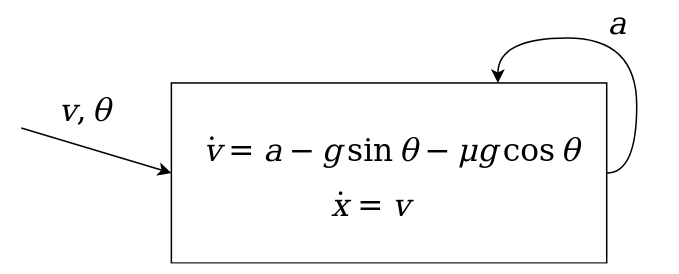
\includegraphics[width=8cm, keepaspectratio]{img/2_1_hybridmod.png}
	\caption{This hybrid model handles the problem of the cruise control. It has only one state and takes as input the vehicle's velocity $v$ and the road's steepness $\theta$. It gives as output the acceleration $a$ that updates the state of the system. The other terms that appear are constants: $\mu$ is the friction constant and $g$ is the gravity.}
\end{figure}


\subsection{Modelling and Design}
The modelling of the continuous part consists in obtaining the equations that appropriately describe the behaviour of the \textit{plant}.
With the aim of deriving the equations involved in the problem, we need to consider the relevant dynamics that take place into our setting.
Once we obtain the differential equations that describe the system, we can make some considerations on its controllability and, in particular, on the way the control should occur.

The modelling of the discrete part, instead, aims at identifying the possible discrete \textit{controller}'s states.
This procedure is fundamental to obtain the FSM that can completely represent the \textit{controller}.
The implementation of the FSM as an algorithm is often not-trivial due to the many machine's limitations: memory, compute power, precision and execution's speed are all finite resources.

In particular, the last constraint has become an important bottleneck that is preventing CPS from scaling massively \cite{realtimecps}.
When designing a controller, in fact, it's very important to take into account the latency that will occur between the moment in which the sensors will get information about the state and the moment in which the actuators can react accordingly, after that the \textit{controller} has determined the strategy to follow.
In \textit{time-critical} systems this latency should be kept as low as possible in order to keep the system into a safe state and deliver the response action in time.
Traditional methods are still able to stand out with respect to the newer counterparts due to the fact that the most sophisticated control techniques require complex algorithms that, sometimes, cannot run fast enough to make the system a \textit{real-time} one \cite{pidrulez}.

A fundamental part of the design process consists in paying attention to the kind of feedback we expect to receive from the system once that the planned action has taken place through the actuators.
There are two possible choices: designing an \textit{open-loop system} or a \textit{closed-loop system}.

In an \textbf{open-loop} system there is lack of feedback: there is no way for the controller to check whether a given action actually took place or not.
Of course the limits of this approach are evident but they can work reasonably good in certain scenarios.
Examples of \textbf{open-loop} systems are many appliances that, once that they have been instructed on what to do, they execute the program and terminate.
On the other hand, the advantages are lower complexity and fewer resources needed.

A \textbf{closed-loop} system, instead, is characterized by the feedback's presence right \textbf{after} the action has occurred.
The purpose of the feedback is to check whether the action actually brought the system into the desired state or if it still needs more operations in order to reach it.
These kind of systems are \textit{adaptive} and more reliable respect to the \textit{open-loop} ones since they can detect unexpected behaviours and handle them adequately.
By contrast, these kind of systems are more expensive since they require specific sensors and control algorithms in order to provide the feedback.

\begin{figure}[H]
	\centering
	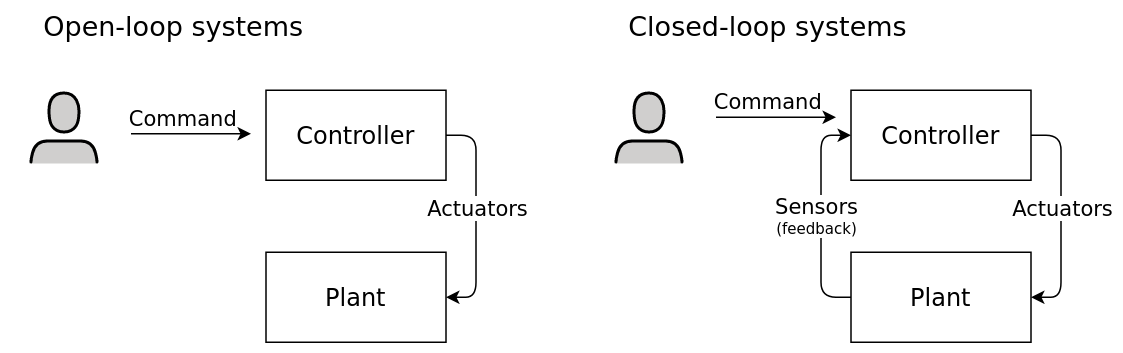
\includegraphics[width=12cm, keepaspectratio]{img/2_1_openclosed_loop.png}
	\caption{Illustration of the difference between open-loop systems and closed-loop systems. The term closed-loop refers precisely to the circular communication that is present in the system.}
\end{figure}

Once we have modelled the whole CPS, it is possible to build software simulators of both the continuous and discrete dynamics in order to test the performance and the capabilities of the system.

\subsection{Safety and monitoring}

The interest in CPS is steadily growing, and as such the research landscape of CPS is complex and rich \cite{Greer2019CyberPhysicalSA}.
One theme receiving a lot of attention is that of CPS \textit{safety} and \textit{security}.
While \textbf{security} is about preventing malicious attacks of the CPS \cite{cps_sec}, \textbf{safety}, in particular, concerns the behaviour of CPS and their interaction in an open world, which should be safe and not lead the CPS device or other interacting agents -- especially humans -- to accidents. 
Safety can be framed in a formal setting by requiring a CPS to satisfy a given set of formal requirements, describing in a mathematically sound way properties like "the autonomous vehicle never bumps into a human" or "the vehicles's speed should always remain close to $50km/h$", in the case of the cruise-control.

A popular language to specify safety properties is Signal Temporal Logic \cite{stl2004}, a \textit{temporal logic} tailored to deal with continuous quantities that we are going to cover more in detail in the last section of this chapter. 
Given a STL property, in principle, we would like to formally verify that it holds for the CPS under consideration, or at least for its mathematical model.
This means having a formal proof that each trajectory of the model is safe.
Such procedure is named \textbf{verification} or \textbf{model checking}.
Verification of STL properties on hybrid systems, however, is often undecidable or just computationally too complex -- especially in the case of \textit{stochastic models} -- therefore it is an active field of research \cite{Zheng_Julien_2015}.

In such cases a common approach is that of \textbf{monitoring} the system trajectories at \textit{run-time} with STL properties and leveraging this information to assess safety in a weaker way, e.g. only with statistical guarantees. 

Another technique to assess the safety of a CPS is \textbf{falsification}.
This technique applies \textit{monitoring} to simulations specifically conceived in order to drive the system to an unsafe state \cite{cps_falsification}.
STL propositions are used to identify the dangerous corner-cases that can be used as \textit{counterexamples} for gaining insight on how the problem occurred and to tune the model's parameters accordingly \cite{counter-tuning} or to train the model to avoid such cases \cite{counter-train}.


\section{Generative Adversarial Networks}

A Generative Adversarial Network (GAN) is a \textbf{generative model}, a class of statistical models whose aim is to learn the probability distribution of the input data.

In particular, this family of models learns a mapping function between a given distribution $P_z$ and the distribution learnt from the data $P_{latent}$.
The learning procedure is supervised and aims at reducing the difference between the generative distribution $P_{latent}$ and the dataset distribution $P_{data}$.
A peculiar characteristic of these models is that, once the learning procedure has been completed, it is possible to sample from them using the noise distribution $P_z$.

Summarizing, a generic \textit{generative model} takes as input a noise vector $z \sim P_z$ and maps it to a sample drawn from the distribution $P_{latent}$, learnt from the data distribution $P_{data}$.
The term "generative" refers to the capability of the model of \textbf{generating} new artificial samples that resemble the provided ones.

GANs, in particular, use NNs and a specific learning approach in order to learn the mapping function between the two distributions.
In the following sections we are going to cover the concepts used by GANs.

\subsection{Neural Networks}
The concept behind Neural Networks (NNs) is quite old despite only in the last decade the related literature is flourishing \cite{nn_survey}.
This is happening because of the availability of \textit{big data} and the increased computational power allow a faster and more accurate training, allowing their employment to deal with increasingly complex problems.
The ancestors of the modern NNs root their history in the '50s, when scientists begun understanding and formalizing how biological neurons work \cite{Rosenblatt58theperceptron}.

\subsubsection{Perceptron}
The term \textit{perceptron} was coined during the '50s and its way of working was already incredibly similar to how modern NNs work.
Since the \textit{perceptron} can be considered an ancestor of the NNs of today and they still have a lot in common, we'll describe how a simple \textit{perceptron} works.

The whole \textit{perceptron} can be represented by a function that takes a vector of inputs $\Bar{x}$ and gives a binary output.
For each input the perceptron has one internal parameter called \textbf{weight} denoted by $\Bar{w}$ and a \textbf{bias} term $b$, that encodes the prior knowledge.
The \textit{perceptron} does one very simple thing: it \textit{weights} the external input $\Bar{x}$ with the internal parameters $\Bar{w}$, it sums them up along with $b$ and it applies to the result an \textit{activation function} that determines the final output of the \textit{perceptron}.
Nowadays \textit{non-linear activation functions} are the most used although there is a vast literature about them \cite{nwankpa2018activation}.

The activation function of the perceptron is called Heaviside -- a simple step function -- and is defined as follows:
\[ act(z) = \begin{cases} 
      1 & z \geq 0 \\
      0 & z < 0 
   \end{cases}
\]

The output of the single perceptron will be given by
$$
act(b+ (\Bar{x}^T \Bar{w})) = act \left(b+ \sum_{i=1}^{n} x_i w_i \right)
$$

\begin{figure}[H]
	\centering
	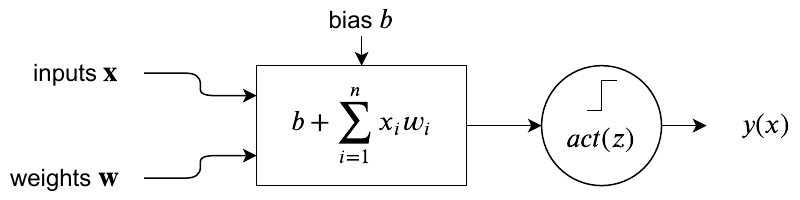
\includegraphics[width=8cm, keepaspectratio]{img/2_2_perceptron.png}
	\caption{Schematic view of the perceptron.}
\end{figure}

This definition is inspired by biological neurons and their electrophysiology: they receive some inputs, combine them and then, through the equivalent of the activation function, decide whether or not to propagate the signal \cite{Rosenblatt58theperceptron}.

\subsubsection{Deep Neural Networks}
Like in the animal brains, we can achieve interesting flexibility of the model when we link multiple perceptrons together.
In particular, during the years the community started following the approach of structuring the NNs in a layered fashion \cite{layered_nets} although, in the recent years, researchers are exploring new ways of optimizing and structuring differently the NNs to gain in performance \cite{lottery_ticket} \cite{weight_agnostic}.

\begin{figure}[H]
	\centering
	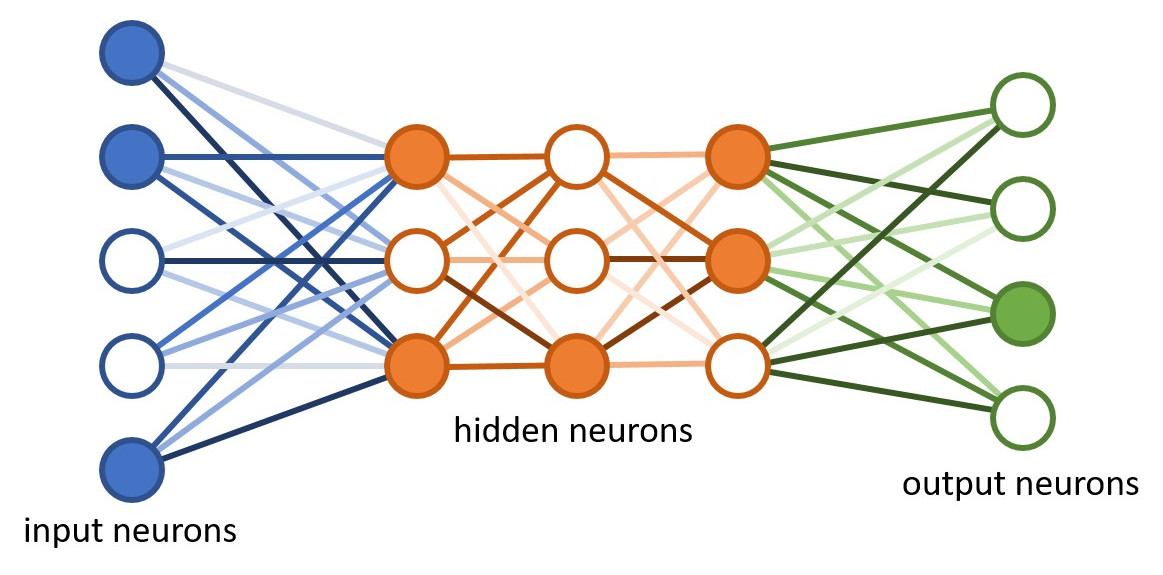
\includegraphics[width=12cm, keepaspectratio]{img/2_2_dnn.jpeg}
	\caption{Schematic representation of a Deep Neural Network ans its layers.}
\end{figure}

What makes a neural network "deep" is actually the number of layers between the \textit{input layer} and the \textit{output layer} of the network.
These layers are called \textit{hidden}.
In a layered NN, the outputs of the previous layer are the inputs to the next layer.
With the exception of a few more sophisticated structures, NNs usually form an acyclic graph, known as \textit{feed-forward network}.

It can be proven that a NN is a \textit{universal approximator} of functions \cite{hornik1989multilayer}, this means that it is possible to approximate with arbitrary precision any measurable function depending on the number of neurons present in the NN.
It is worth mentioning that choosing a \textit{non-linear activation function} allows the NN to approximate even \textit{non-linear} behaviours.
This is usually a common practice, especially when using DNN.

\subsubsection{Training of a Neural Network}
What makes the NNs so relevant is the learning procedure that is used to train them.
The vast majority of the NNs, in fact, make use of \textit{supervised learning} \cite{liu2017survey} in order to adjust the internal parameters and, therefore, learn to approximate a given function.
The term "supervised" means that the model learns being exposed to many labelled examples.
For instance, let $D$ be a training set $\{(\Bar{x}_1, y_1), \dots, (\Bar{x}_n, y_n)\}$ of arbitrary length $n$.
Each element of the set is composed of a feature vector $\Bar{x}_i$ and the respective label $y_i$.
The training procedure allows a generic NN to learn the underlying structure that links the input to the output, in the case of the training set $D$, how to map each feature vector $\Bar{x}_i$ to the respective label $y_i$.

As an example, let $f$ be a NN with one layer only, a function of the input vector $\textbf{x}$ and the matrix of its weights $\textbf{W}$ that gives us, as output, the predicted values.
The vector notation for NNs naturally extends the one of a single perceptron:
$$ f(\textbf{x}, \textbf{W}) = act(\textbf{W} \textbf{x}) $$

Let us take a generic training dataset composed by row vectors $\textbf{x}_i$ of predictors and the respective vector $\textbf{y}_i$ of the dependent variables.
Since we are in the context of \textit{supervised learning}, once the full training is completed, we would expect that our neural network has learnt how to map $\textbf{x}$ to $\textbf{y}$.
Let us provide our NN $f$ the training example $\textbf{x}$, we obtain the predicted value $\hat{\textbf{y}}$:
$$ f(\textbf{x}, \textbf{W}) = \hat{\textbf{y}} $$

We initialize the weights $\textbf{W}$ of the NN randomly and, therefore, the predicted $\hat{\textbf{y}}$ will not be very close to the desired value $\textbf{y}$.
The training procedure tunes the internal weights $\textbf{W}$ in such a way to make the predicted value $\hat{\textbf{y}}$ as close as possible to the true label $\textbf{y}$.

We introduce the concept of \textit{loss function}, that is a measure of the difference between $\textbf{y}$ and $\hat{\textbf{y}}$ or, in other words, the prediction error of the NN.
An common example of \textit{loss function} is the \textit{Mean Squared Error}:
$$ \mathscr{L}(\textbf{y}, f(\textbf{x}, \textbf{W})) =
\mathscr{L}(\textbf{y}, \hat{\textbf{y}}|\textbf{W}) =
\frac{1}{n} \sum_{i=1}^{n} (\textbf{y}_i - \hat{\textbf{y}}_i)^2 $$

$\mathscr{L}$ depends on the weights $\textbf{W}$ of the NN, therefore we can minimize it w.r.t. the weights $\textbf{W}$ and find the optimal ones for the provided training examples.
Minimizing such \textit{loss function} is not easy due to the high dimensionality of the problem and the underlying high non-linearity.
The standard procedure that set a turning point in the world of NNs and that helps to solve efficiently this problem is called \textbf{backpropagation} \cite{Rumelhart1986}.

The backpropagation algorithm computes, for each unit of the NN, the derivative of the error with respect to the weights $ \frac{\partial \mathscr{L}}{\partial w_{ij}} $ in order to come up with the \textit{gradient} of the error.
Once the \textit{gradient} has been computed, we use an \textit{optimization algorithm} that minimizes the error and updates the weights of the NN accordingly.
A very common example of \textit{optimizer} is \textbf{Stochastic Gradient Descent}, which searches for the optimal parameters in the directions where the \textit{gradient} is lower.
The stochasticity is used to add noise to the trajectory and to avoid getting stuck into a local minima \cite{zhang2004sgd}. 

The training procedure is repeated until the NN reaches the desired performances.


\subsection{Zero-sum games}
Before analyzing a GAN, we should first introduce some concepts borrowed from Game Theory useful in games with \textit{non-cooperative} setting.
The term "adversarial" comes, in fact, from the peculiar competitive interaction that takes place inside GANs' architecture.
In a non-cooperative settings with two players, for instance, a zero-sum game is a kind of game in which, whenever a player wins an specific amount the other player looses the same amount.
Basically players can only steal each others' reward, this is the reason behind the expression \textit{zero-sum}.

This concept is fundamental because it states that there's no other way of maximizing the individual gain without penalizing the other player.
Othewise, in the case of a \textit{non-zero-sum game},  players would not be forced to to overcome the opponent anymore and it would be possible to find other kind of strategies to increase the individual gain.
Instead, it is fundamental, in the context of GANs, that we keep the setting competitive.

Coming back to the \textit{zero-sum games}, the best winning strategy for each player is to apply the \textbf{minimax} strategy.
Let $V$ be the \textit{value function} that computes the expected reward given the choices of the players $a$ and $b$, we define the maximum loss as the $ \inf \{V(a,b)\}$.
The objective of both the players becomes the\textit{mini}mization of the \textit{max}imum loss.
In particular, the strategy of a player $a$ playing against $b$ is:
$$ \underset{a}{\text{min}} \; \underset{b}{\text{max}} \; V(a,b) $$

If both players played according to the minimax strategy, they would end up in a stable state of their choice: the choice of each player would no longer depend on the opponent's choice since the optimal strategy would have been found and any change to this choice would not improve the payoff.
This situation happens because, being a \textit{zero-sum game}, the best strategy is to choose the action the maximizes the personal reward assuming that the opponent is playing at its best.
This peculiar situation in which the dominant strategy is found by the two players, it is called \textit{Nash equilibrium}.

As we will see, this is a core concept for a GAN.


\subsection{Description of a GAN}
GAN architecture is composed by two NNs that play against each other in a zero-sum game \cite{gan_2014}.

The typical terminology used in GANs refers to the two architecture's NNs naming them \textbf{generator} and \textbf{discriminator}.

The \textbf{generator} is a NN $G(\textbf{z}, \theta_G)$ where $\theta_G$ indicates the network's parameters and $\textbf{z}$ is a noise vector drawn from a given prior distribution $P_z$.
$G$ is a \textit{generative model} that tries to learn the mapping between $P_z$ and the distribution $P_G$ learnt from the data distribution $P_{data}$.
The output of $G$, given $z \sim P_z$, is a sample of the distribution $P_G$.
This sample, coming from the estimated distribution $P_G$, will resemble the samples drawn from the data distribution $P_{data}$.

The \textbf{discriminator} is a NN $D(\textbf{x}, \theta_D)$ where $\theta_D$indicates the network's parameters and $\textbf{x}$ is a vector of data.
$D$ is a \textit{classifier} that outputs the probability for the vector $\textbf{x}$ to come from the training distribution $P_{data}$ or from the learnt distribution $P_G$.

\begin{figure}[H]
	\centering
	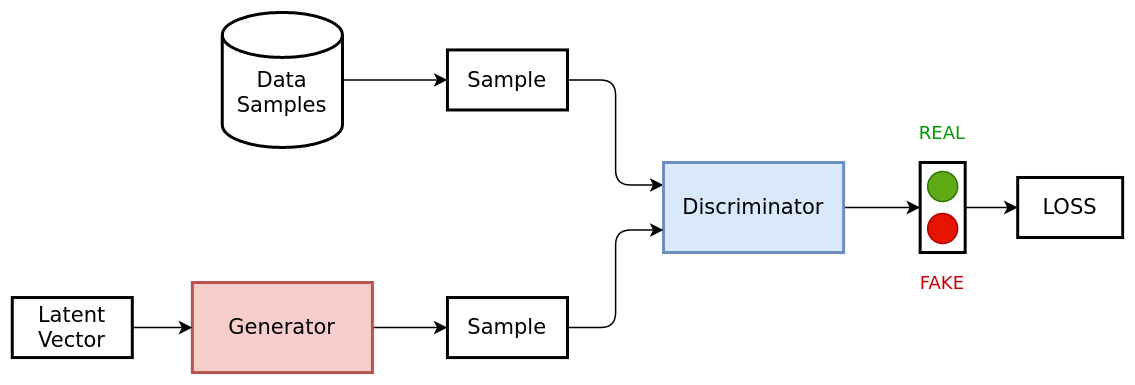
\includegraphics[width=12cm, keepaspectratio]{img/2_2_gan_arch.png}
	\caption{Schematic architecture of a GAN.}
\end{figure}

It should be clear by now that the two networks of the GAN have opposing roles.
The aim of the \textit{generator} is to produce data samples that resemble the true data distribution and, consequently, to fool the \textit{discriminator} leading it to a \textit{false-positive} classification.
On the other hand, the aim of the \textit{discriminator} that of classifying correctly as much data vectors as possible.
The two NNs are bound to this non-cooperative zero-sum game by the following \textbf{minimax} game:
$$ \underset{G}{\min} \; \underset{D}{\max} \; V(G,D) = \mathbb{E}_{x\sim p(x)}\big[\log(D(x))\big] + \mathbb{E}_{z\sim p_{z}(z)}\big[\log(1-D(G(z)))\big] $$

From the formula we can observe how $D$ tries to maximize the number of correct classifications of the original data -- the part $\log(D(x))$ -- and the generated data -- the part $\log(1-D(G(z)))$ -- while $G$, on the other hand, by tuning its internal parameters $\theta_G$, tries to minimize the number of correctly classified fake images producing more likely results.
From the formula above it is possible to derive the individual \textit{loss functions} that can be adapted to the specific problem's domain \cite{gan_loss_survery}.

Both the NNs are trained in turns and, when one NN is learning, the parameters of the other are kept constant.
Both training procedures take place as described above: starting from the \textit{loss function}, the \textit{gradient} is computed through \textit{backpropagation} and the network's weights are updated by the \textit{optimizer}.

Theoretically, after the training, the two NNs should reach the \textit{equilibrium} so that the \textit{generator} should be able to precisely mimic the data distribution $P_{data}$ and the \textit{discriminator} would guess randomly whether the presented sample is fake or not.

\subsection{Usage of GANs}
The GANs have been considered one of the most innovative idea in the field of DNNs.
Nowadays, they have many applications, especially where image manipulation is involved.
GANs, in fact, are particularly successful in the task of generating or modifying images.
For this reason GANs are usually associated with \textbf{Convolutional} NNs, a particular architecture of NN that is effective in dealing with images \cite{dcgan}.

\begin{figure}[H]
	\centering
	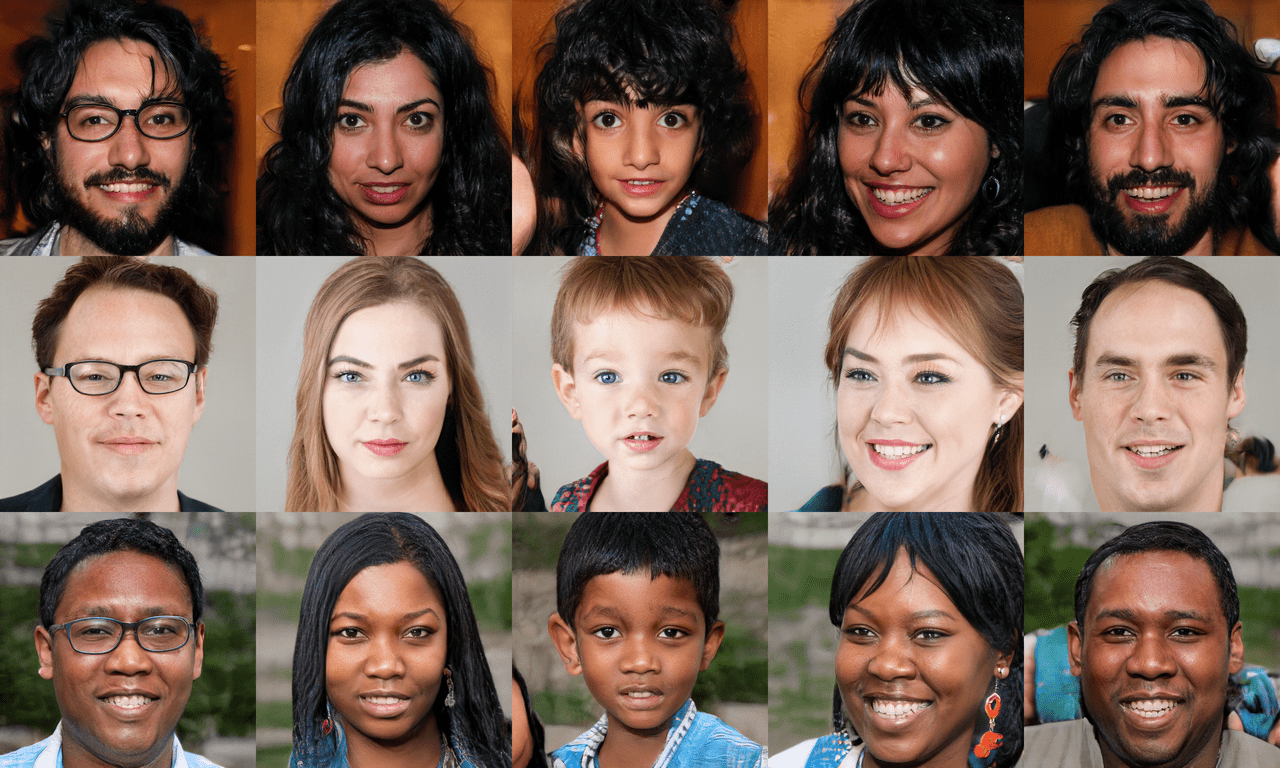
\includegraphics[width=12cm, keepaspectratio]{img/2_2_stylegan_faces.png}
	\caption{The faces above are artificially generated by StyleGAN.}
\end{figure}

Some innovative applications include:

\begin{itemize}
  \item Image super-resolution \cite{superres}, to increase the resolution and details of low resolution images
  \item Image inpainting \cite{inpainting}, to reconstruct masked/missing parts of one image
  \item Paint to image \cite{paintimg}, from a sketch or a simple paint they can reconstruct a picture
  \item Data synthesis \cite{datasynth}, used to produce synthetic samples of images similar to the ones of the training set
  \item Style transfer \cite{CycleGAN2017}, used to apply to a picture the artistic style of a given drawing
  \item Image harmonization \cite{harmonization}, to blend seamlessly two images or parts of them
\end{itemize}

\begin{figure}[H]
	\centering
	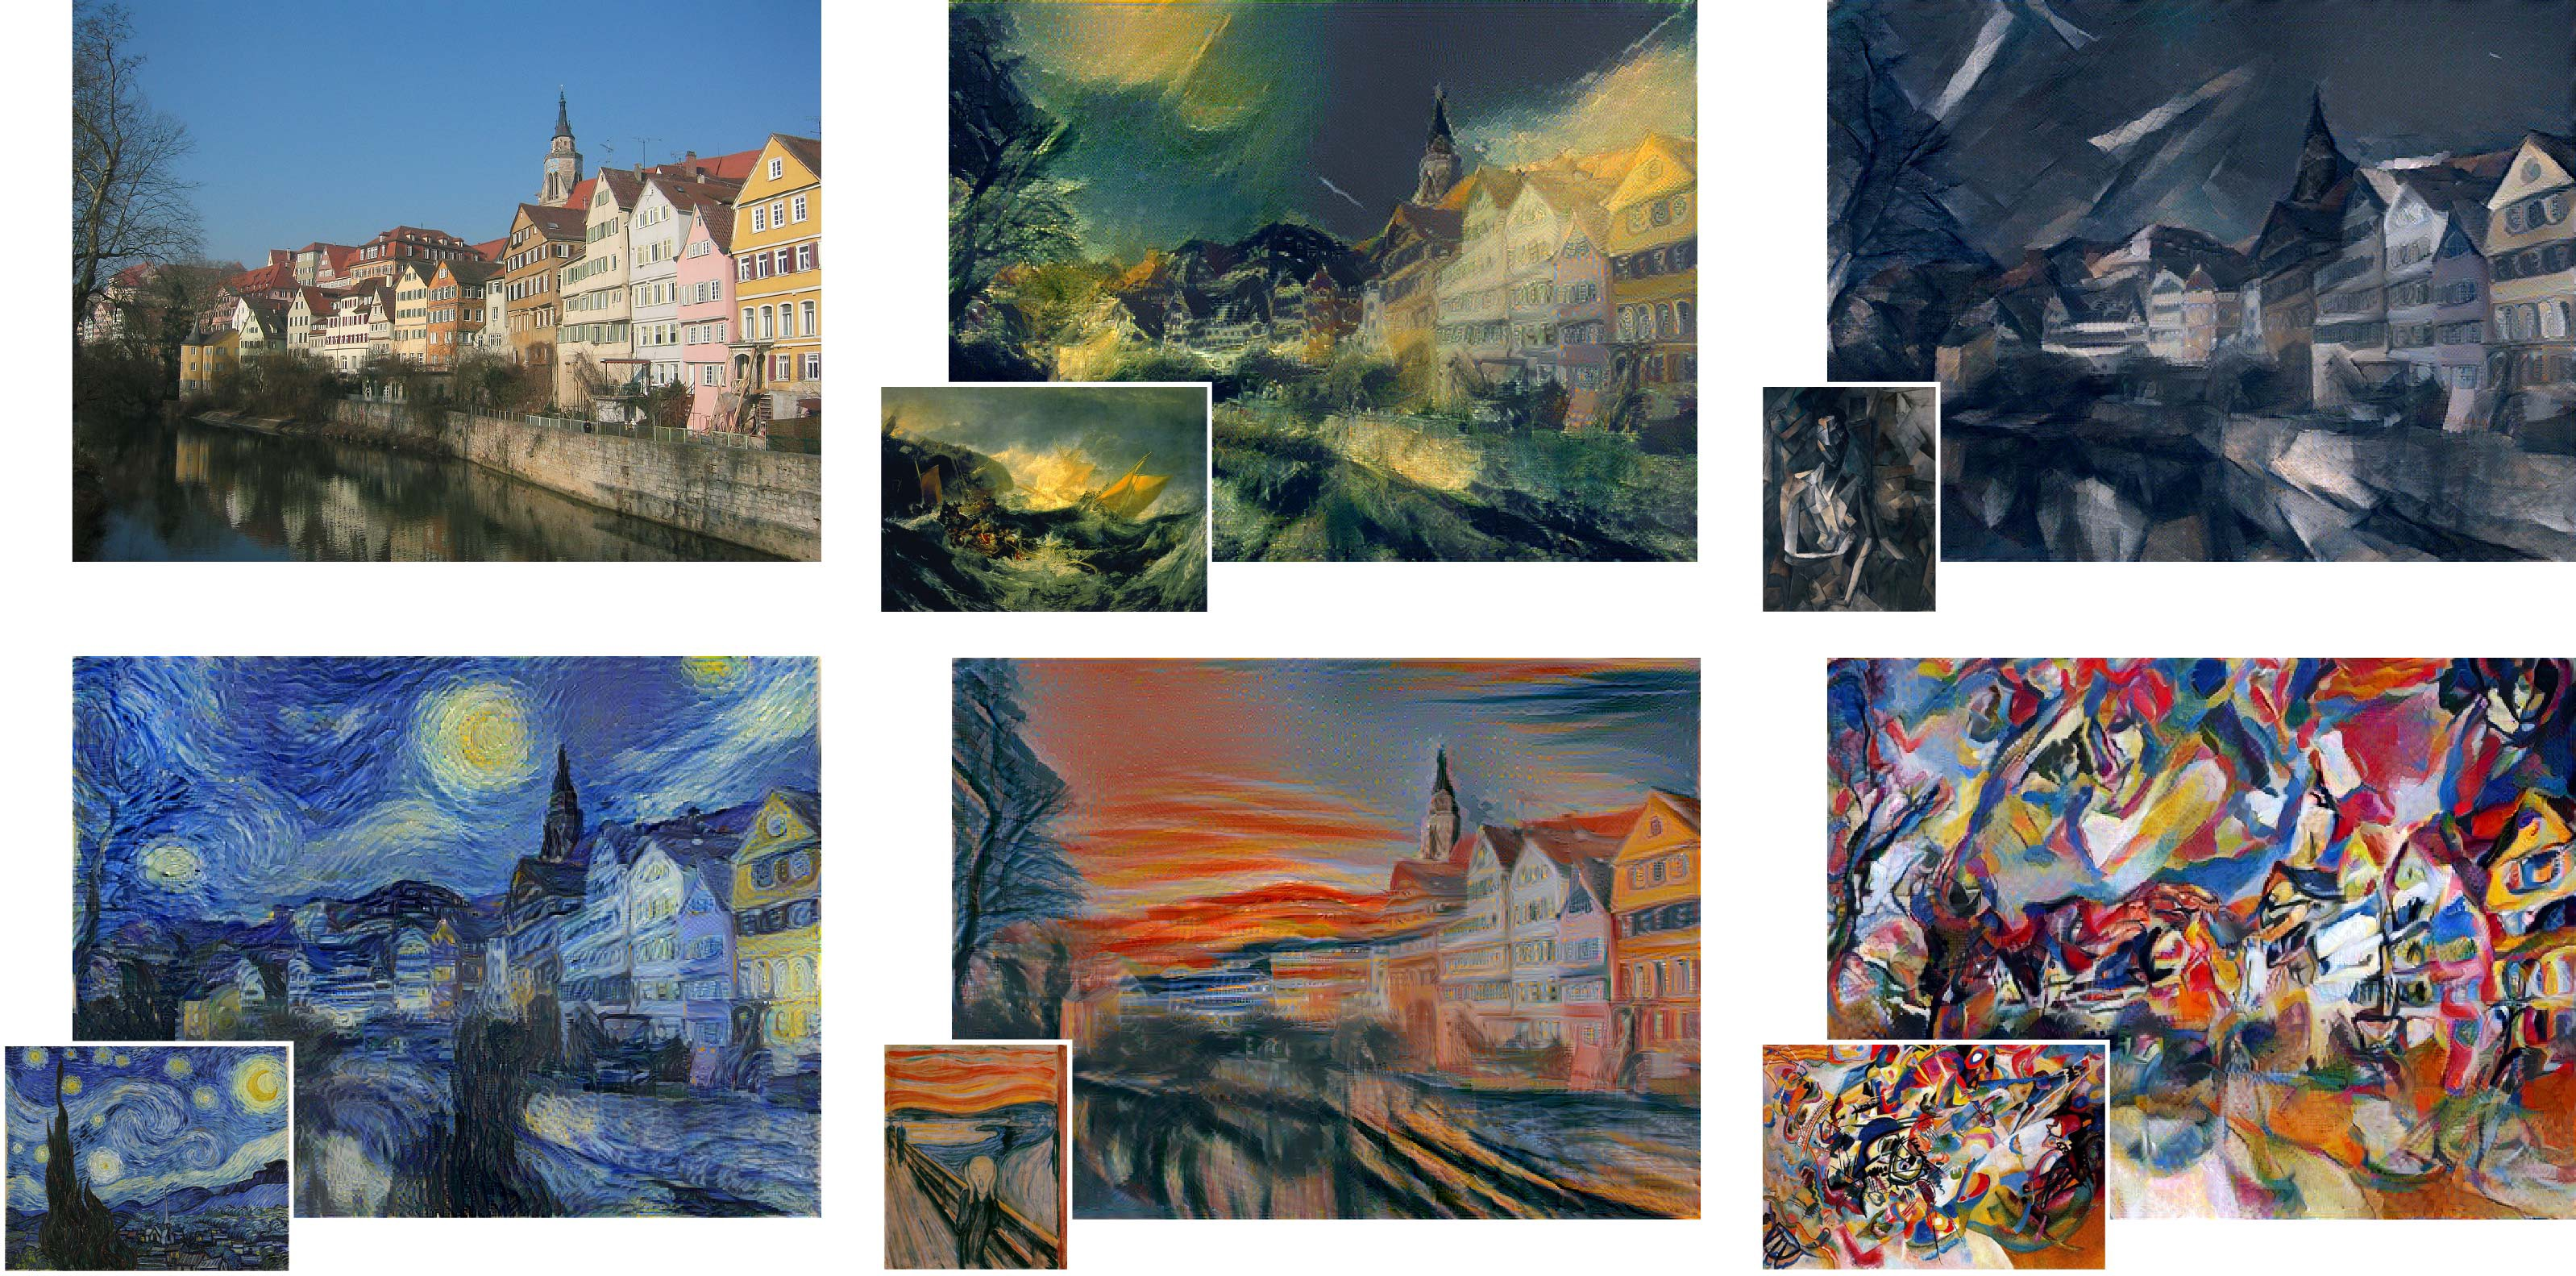
\includegraphics[width=12cm, keepaspectratio]{img/2_2_styletransfer_paintings.jpeg}
	\caption{Examples of Neural Style Transfer: a GAN trained to extract the stylistic features of paintings to apply them on pictures.}
\end{figure}

This was just a quick overview of the most promising applications of the GANs.
The research area around them is very vivid and in rapid evolution.
The power and the credibility of such technologies became so high that they started to rise some concerns due to malicious and immoderate usage \cite{tolosana2020deepfakes}.

\section{Signal Temporal Logic}

\textit{Temporal Logic} (TL) is mostly known for the formal verification of models, both hardware and software.
It was conceived to check a discrete signal measured over time against a logical proposition that makes use of special operators.

The term \textit{Temporal Logic} refers to a broad family of logics used for formal verification.
Each temporal logic follows precise rules on how to build the propositions using the allowed operators.
The aim is to analyze and check some requirements for a given \textit{time series}.
TL relies on a basic set of \textit{temporal operators} used to deal with time-related variables \cite{sep-logic-temporal}.
They are used in formal verification to assign a \textit{truth value} to a given \textit{time series} according to the properties expressed by the TL statement.

We are going to cover in detail only one kind of \textit{Temporal Logic}, the \textbf{Signal Temporal Logic} (STL).
This logic has been created to deal with continuous-time signals by discretizing them \cite{stl2004}.

\subsection{Syntax}
The basic component of a STL statement is the \textbf{atomic predicate}, generally named $\mu$.
Let $s$ be a generic signal over time $t$, an \textit{atomic predicate} $\mu$ is a logical function of the signal, i.e. $\mu = f(s(t)) > 0$ where $f$ is a generic function defined over the signal's state space $\mathcal{S}$, $f: \mathcal{S} \to \mathbb{R}$ .

STL syntax allows to chain multiple atomic predicates by means of the \textbf{operators} to obtain a STL proposition, generically referred to as $\varphi$.
The operators defined in STL are \textit{logical} or \textit{temporal}.
\textit{Logical operators} are the very same used in every logic: negation $\neg$, and $\wedge$, or $\vee$.

The \textbf{temporal operators} are introduced specifically in TLs and are used to check properties of the signal over time.
The \textit{temporal operators} defined in the STL syntax are: $\mathcal{G}$\textit{lobally}, $\mathcal{F}$\textit{inally} and $\mathcal{U}$\textit{ntil}.
The operator is referred to as \textit{bounded} if it is defined over a finite \textit{interval}, otherwise it is \textit{unbounded}.

An \textbf{interval}defines the time window in which a given operator is applied.
For instance, the notation $[0,H]$ denotes all the possible intervals $(t_i, \dots, t_{i+H})$ in the time $t = (t_0, t_1, \dots, t_n)$ over which the signal $s$ is defined.
The operator paired with a specific interval operates on the specified sliding window.
Sometimes we refer to $\mathcal{I}$ as the generic interval $\mathcal{I} = [a,b]$.

The notation for specifying a \textit{bounded operator} over the proposition $\varphi$ is, for instance, $\mathcal{G}_{[a,b]}\varphi$.
These operators specify how the given condition $\varphi$ should be evaluated with respect to the timeframe specified by the interval $[a,b]$.

Giving an intuitive explanation of the three operators:
\begin{itemize}
  \item $\mathcal{G}_{[a,b]}\varphi$: $\varphi$ must always be true within $[a,b]$
  \item $\mathcal{F}_{[a,b]}\varphi$: $\varphi$ must become true at least once within $[a,b]$
  \item $\varphi_1\mathcal{U}_{[a,b]}\varphi_2$: $\varphi_2$ must become true
at least once within $[a,b]$ and $\varphi_1$ must be always
true prior to that time
\end{itemize}

The rules of the grammar STL uses to create any formula $\varphi$ can be encoded in a very compact way:
$$ \varphi := \top \;|\; \mu \;|\; \neg\varphi \;|\;
\varphi_1 \lor \varphi_2 \;|\; \varphi_1 \mathcal{U}_{[a,b]} \varphi_2 $$

From the operator $\mathcal{U}$, it is possible to derive the other two operators, $\mathcal{F}$ and $\mathcal{G}$:
$$ \mathcal{F}_{[a,b]}\varphi = \top \mathcal{U}_{[a,b]}\varphi
\qquad \text{and} \qquad
\mathcal{G}_{[a,b]} = \neg\mathcal{F}_{[a,b]}\neg\varphi $$


\subsection{Boolean semantics}
Given the STL syntax, we can give a specific meaning to each symbol.
As we already said, the temporal logics have been created to \textit{verify} some properties and, in case of STL, signals.
The term "verification" implies the computation of a \textit{truth value}, in fact, the most natural semantics that a STL formula can have is the \textbf{Boolean semantics}.

Let $s$ be the signal defined over time $t$ and let $\varphi$ be a STL statement built to express a requirement on $s$.
The \textit{Boolean semantics} allows to \textit{check} whether a given signal $s(t)$ satisfies or not the requirements expressed by the STL proposition $\varphi$.
The satisfaction of the formula $\varphi$ is expressed by the \textit{truth value} assigned by the semantics to the specific signal $s(t)$.

It is possible to define recursively the \textit{Boolean semantics} of STL:
\begin{align*} % notation from https://arts.units.it/retrieve/handle/11368/2856192/69577/RV15-post.pdf
 (s,t) \models \mu \iff & f(s(t)) = 1 \\
 (s,t) \models \neg \varphi \iff & (s,t) \not\models \varphi \\
 (s,t) \models \varphi_1 \vee \varphi_2 \iff & (s,t) \models \varphi_1 \;\text{or}\; (s,t) \models \varphi_2 \\
 (s,t) \models \varphi_1 \mathcal{U}_{[a,b]} \varphi_2 \iff & \exists t' \in [t+a, t+b] \;\text{s.t.}\; (s,t') \models \varphi_2 \\
 & \text{and}\; \forall t'' \in [t, t'], (s,t'') \models \varphi_1
\end{align*}

The trace $s$ satisfies $\varphi$ if and only if $(s, 0) \models \varphi$.
Starting from the definition of the $\mathcal{U}$ntil operator, as we already mentioned, it is possible to derive the operators $\mathcal{F}$inally and $\mathcal{G}$lobally.

By adding these basic operations to the usual Boolean logic, we obtain the full power of the STL Boolean semantics.
With this semantics it is already possible to monitor a signal to perform verification on it.

\subsection{Quantitative semantics}
Another interesting property of STL is the possibility of attributing different semantics to the same syntax.
A \textbf{quantitative} or \textbf{robust} semantics has been formalized as well \cite{robuststl}.

This semantics uses the same notation and operators of the \textit{Boolean semantics}, but provides a different interpretation of the same formulas.
Let us introduce a function $R$ that given the triplet $(s, t, \varphi)$, computes the \textit{robustness} of the signal $s$ with respect to the proposition $\varphi$.
It is possible to define recursively how the semantics works:
\begin{align*} % notation from https://arxiv.org/pdf/1808.03315.pdf
R(s,t,(f(s) \sim \mu)) = & \begin{cases} \mu-f(s_t) & \sim=\le \\ f(s_t)-\mu & \sim=\ge \end{cases}
\\
R(s,t,\neg \varphi,t) = & -R(s,t,\varphi)
\\
R(s,t,\varphi_1 \vee \varphi_2) = & \max(R(s,\varphi_1,t),R(s,\varphi_2,t) )
\\
R(s,t,\varphi_1 \wedge \varphi_2) = & \min(R(s,\varphi_1,t),R(s,\varphi_2,t) )
\\
R(s,t,\varphi_1 \mathcal{U}_I \varphi_2) = & \underset{t^\prime \in t+I} \max \big (  
 R(s,t,\varphi_2,t'), \underset{t'' \in [t,t']} \min R(s,\varphi_1,t'')\big)
\\
R(s,t, \mathcal{F}_I \varphi) = & \underset{t' \in t+I}\max ~ R(s,\varphi,t') \\
R(s,t,\mathcal{G}_I \varphi) = & \underset{t' \in t+I}\min~  R(s,\varphi,t')
\end{align*}
The \textit{Boolean} and \textit{robust} semantics are tightly related: $R(s,t, \varphi) > 0 \iff (s,t) \models \varphi$ and $R(s,t, \varphi) < 0 \iff (s,t) \not\models \varphi$.

The intuitive idea behind the quantitative semantics is to measure the relative offset between the signal and the given requirement.
This offset represent how much the signal can be shifted before incurring into the change of the truth value for the proposition $\varphi$ and, therefore, into the violation of the constraint.
The \textit{robustness} quantify, in fact, how much variation can be tolerated on the signal.
This property of the semantics makes it particularly suitable for this work.
We are going to use it to measure the \textbf{robustness} of the trajectories proposed by our method.


\begin{figure}[H]
	\centering
	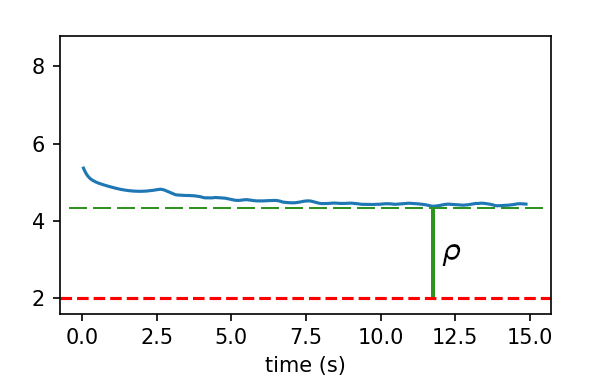
\includegraphics[width=8cm, keepaspectratio]{img/2_3_stl_robustness.png}
	\caption{The quantitative semantics of STL visualized. Let $s$ be the blue signal in the picture and let $\varphi: \mathcal{G}(s > 2)$ be the STL formula that we want to check on it, whose boundary is depicted in red. The robustness $\rho$ represents the offset between the signal and the constraint $\varphi$.}
\end{figure}